\chapter{Experimental Methods \label{cap:exp}}

This chapter details the experimental procedures developed for the fabrication and characterization of photonic networks based on waveguides. The methodology encompasses three fundamental aspects: (1) direct writing of waveguides using a femtosecond laser, (2) optical excitation systems with a supercontinuum laser, and (3) advanced techniques for spatial light modulation to control initial conditions.


\section{Direct Writing of Waveguides \label{cap:fs}}

The fabrication of waveguides was carried out using the direct writing technique with a femtosecond laser: ultrashort pulses emitted from a Yb-doped fiber laser ATSEVA ANTAUS at 1030 nm, with a repetition rate of 500 kHz, are strongly focused into a borosilicate sample, producing slight and permanent changes in the local refractive index $\Delta n \sim 10^{-4}-10^{-3}$. This method, available and implemented by previous members of the Photonic Networks Group, allows for the creation of three-dimensional structures through computer-controlled movements of the Aerotech Nanopositioner XYZ platform \citep{femto_writing}.

\begin{figure}[H]
    \centering
    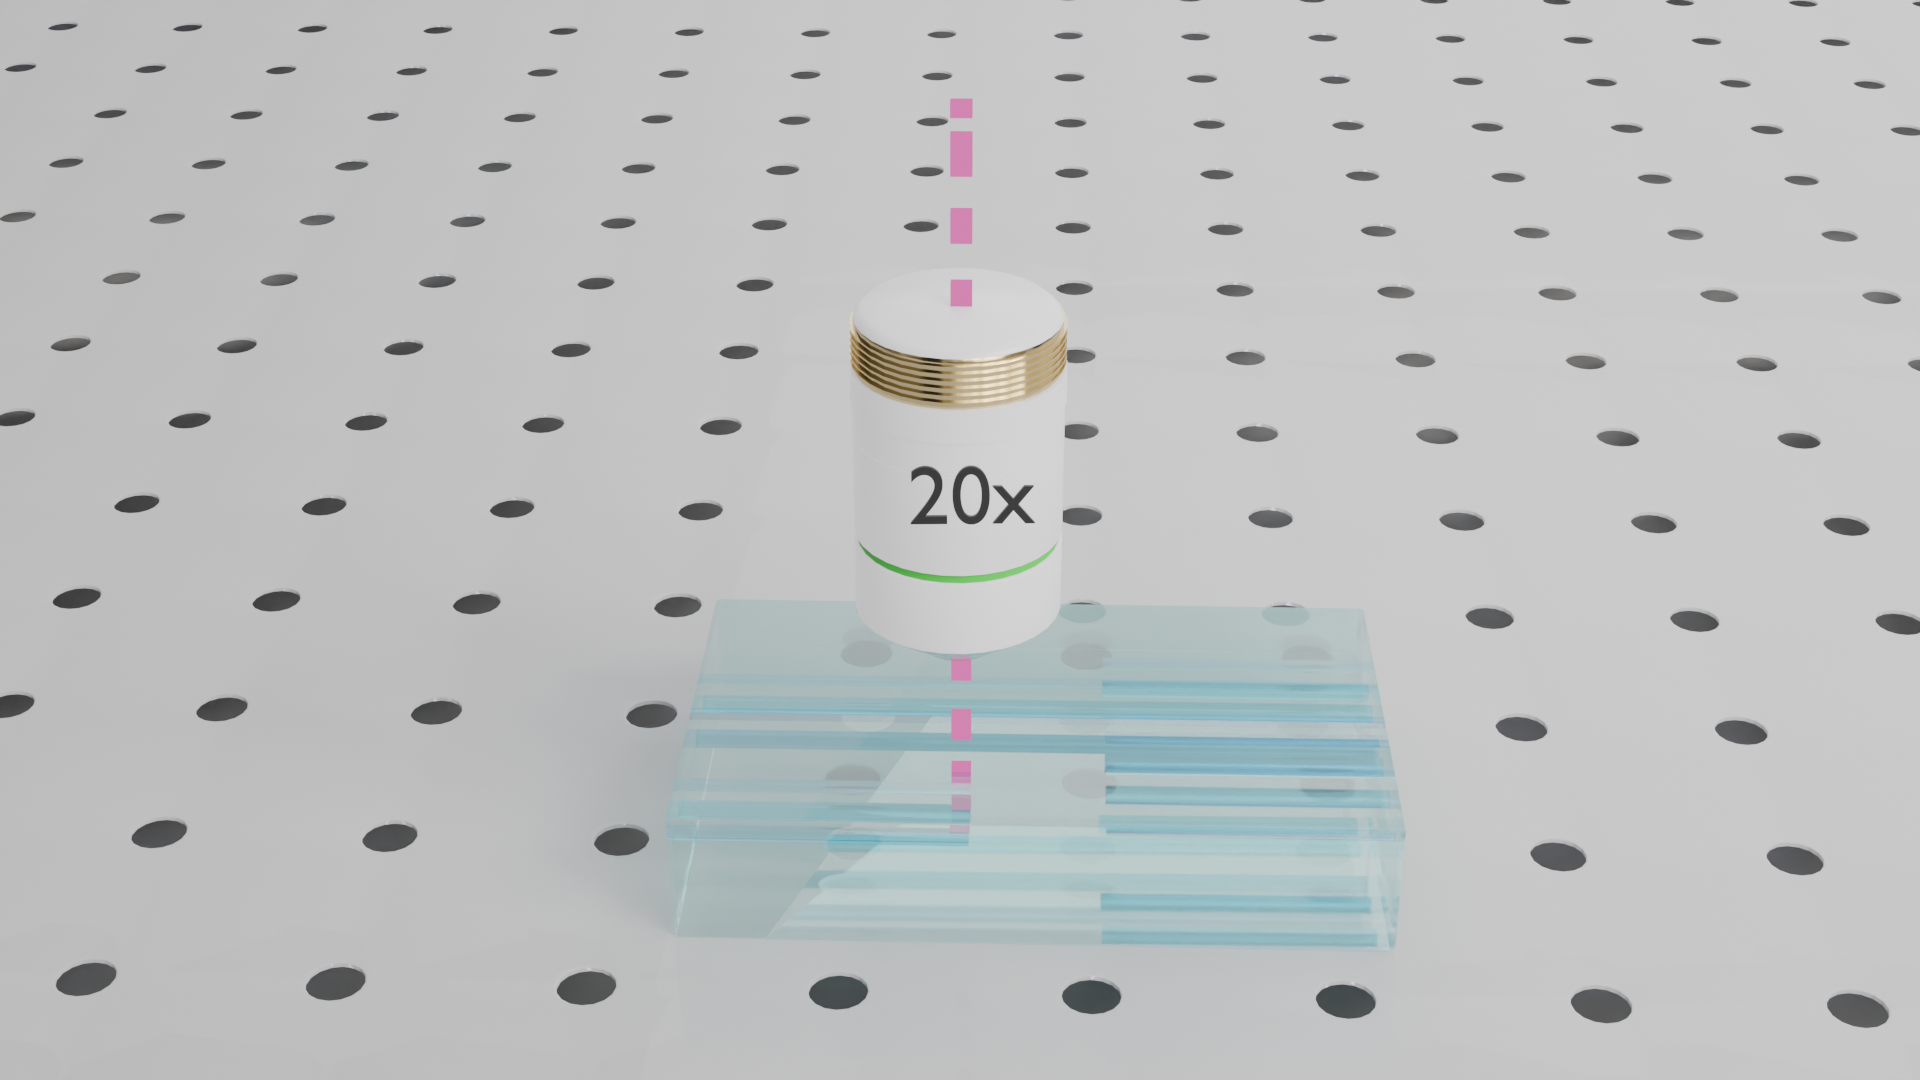
\includegraphics[width=0.5\linewidth, trim={18cm 4cm 15cm 6cm},clip]{media/fabrication1}
    \caption[Schematic of the waveguide writing technique.]{Schematic of the waveguide writing technique. The laser beam is focused using a microscope objective (20x) while the sample is moved along three axes via a computer-controlled platform.}
\end{figure}

The writing parameters that work for exciting modes in the visible spectrum are:
\begin{itemize}
	\item Pulse width: 215 fs.
	\item Repetition rate: 500 kHz.
	\item Writing speed: 0.1 - 20.0 mm/s.
	\item Measured arrival power: 70.0 - 150.0 mW.
\end{itemize}

\section{Supercontinuum Laser Excitation Setup \label{cap:wavelength}}

For optical characterization, an excitation system based on a broadband supercontinuum (SC) laser (470 nm - 2200 nm) was implemented. Specifically, the model is a YSL SC-5. The configuration allows selecting specific wavelengths through an acousto-optic modulator AOTF-PRO (430 nm - 1450 nm), with a spectral resolution of $\pm$5 nm and an output power of 1 mW per wavelength.

\begin{figure}[H]
    \centering
    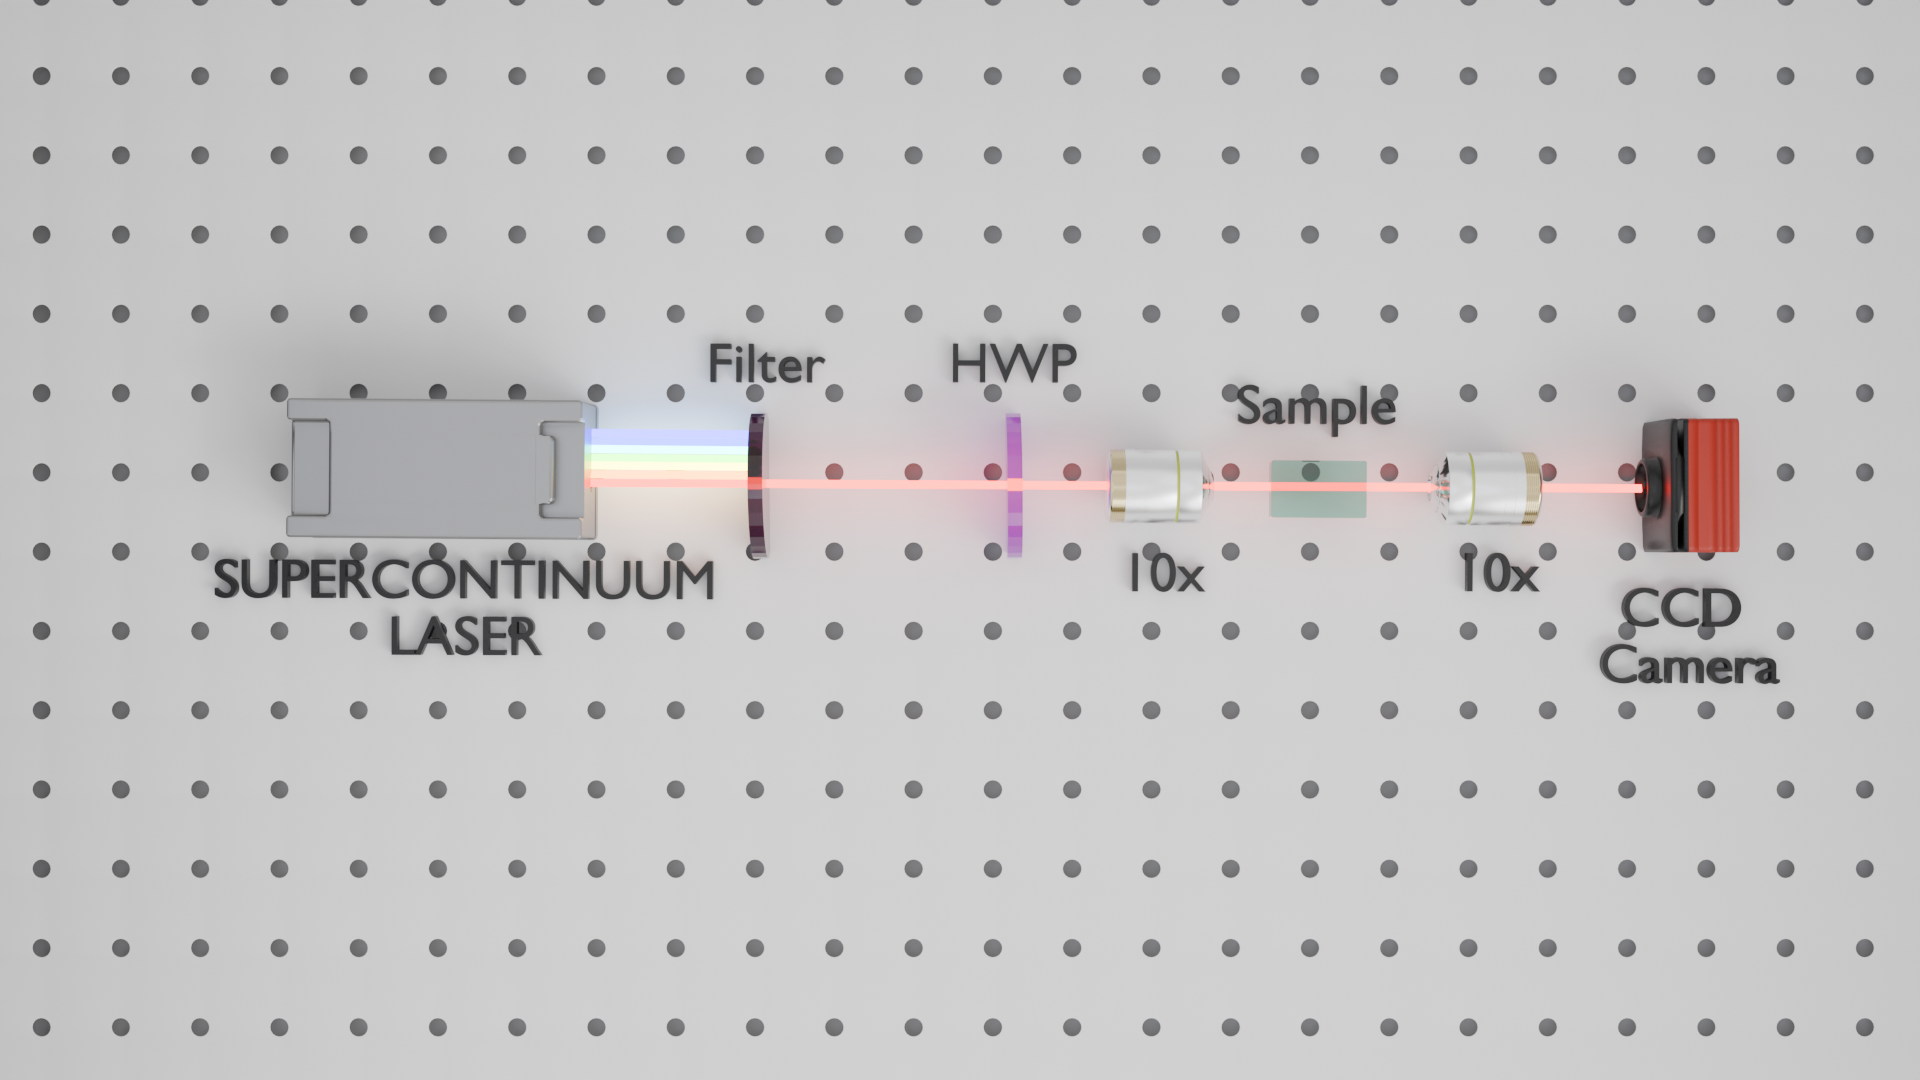
\includegraphics[width=\linewidth, trim={5cm 9cm 3cm 7cm},clip]{media/SC_setup}
    \caption[Supercontinuum laser excitation setup.]{Supercontinuum laser excitation setup. Filter: Acousto-optic modulator and iris. HWP: Half-wave plate.}
\end{figure}

To use initial conditions different from a Gaussian, it is necessary to incorporate methods of spatial light modulation. In this thesis, a technique known as phase encoding via hologram was implemented \citep{terhalle}.

\subsection{Premodulation Stage}
The spatial light modulator used is a HOLOEYE PLUTO-VIS SLM - Reflective LCOS (resolution 1920$\times$080 px, pixel size 8 $\mu$m), whose optical response occurs with polarization parallel to the optical table plane. A half-wave retarder ($\lambda/2$) followed by a Glan-Thompson polarizer 100,000:1 is used to ensure that the laser light polarization matches that of the SLM's response. Subsequently, the beam is magnified and collimated to cover the entire available pixel area using a 20x objective and a 100mm focal length lens (telescope).

\subsection{Modulation Stage}
A diffraction grating that maximizes the power of the first diffraction order is used. To modulate amplitude, the grating must be multiplied by the desired amplitude mask, while for phase modulation it suffices to add the grayscale level corresponding to the desired phase. Figure \ref{fig:SLMblaze} outlines the algorithm implemented in Python in Appendix \ref{sec:codeSLM}.

{
\sidecaptionvpos{figure}{c}
\begin{SCfigure}[]
    \centering
    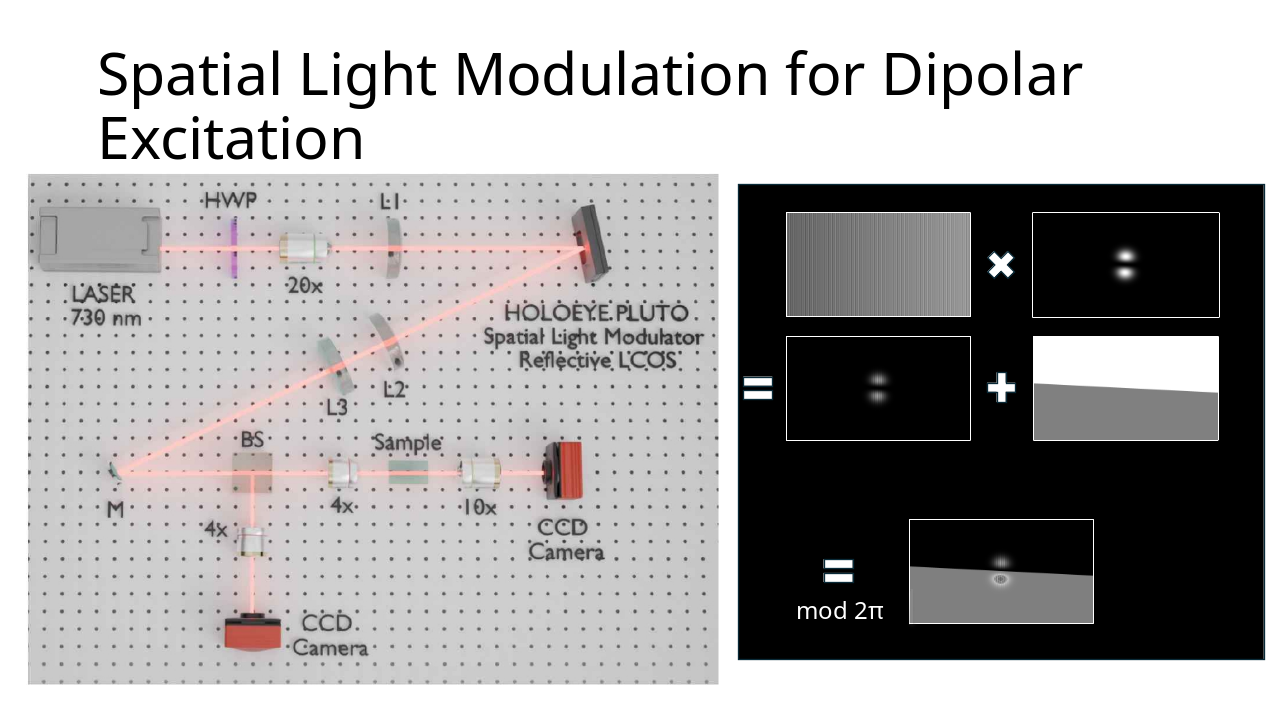
\includegraphics[width=0.35\linewidth, trim={19.5cm 0 0 5cm}, clip]{media/SLMblaze4.png}
    \caption[Spatial light modulation for arbitrary amplitude and phase masks.]{Spatial light modulation algorithm for arbitrary amplitude and phase masks. The diffraction grating parameters are subject to the wavelength used (730 nm).\label{fig:SLMblaze}}
\end{SCfigure}
}

\subsection{Coupling Stage}
The modulated image passes through a pair of lenses, $L_2$  with a 1000 mm focal length and $L_3$ with a 50 mm focal length, to reduce its size to the order of micrometers. The tilt of the sample's input face must coincide with the plane of the modulated image. To achieve this, two pairs of Gaussian beams are generated—one vertical and one horizontal—so that when translating the 4x objective lens, the interference maxima are produced at the midpoint between the centers of the Gaussian beams.

\subsection{Camera Capture Stage}
Once the sample tilt is calibrated, its position is fixed in the experimental setup. The output image is magnified using a 10x objective and captured using a beam profiler (Beam Profiler BC106N-VIS, Thorlabs) with a spatial resolution of 6.45 $\mu$m/px \citep{thorlabs_beam_profiler}.

\subsubsection{Optional Interferometric Configuration}
The setup can be modified to incorporate a Mach-Zehnder interferometer by:
\begin{itemize}
	\item A \textit{beam splitter} between lens $L_1$ and the SLM, using the pre-modulation beam as a reference.
	\item A second \textit{beam splitter} before the camera to recombine the beams.
	\item A neutral density (ND) filter to balance the intensities ($I_{\text{ref}} \approx I_{\text{muestra}}$).
\end{itemize}
For the generation of dipole modes, it is essential to adjust the phase difference between the recombined beams to a value close to ππ. This is experimentally evidenced by the appearance of an intensity minimum at the center of the interference pattern, corresponding to destructive interference in that region.

\subsection{Optical Circuit}
\begin{figure}[H]
	\centering
	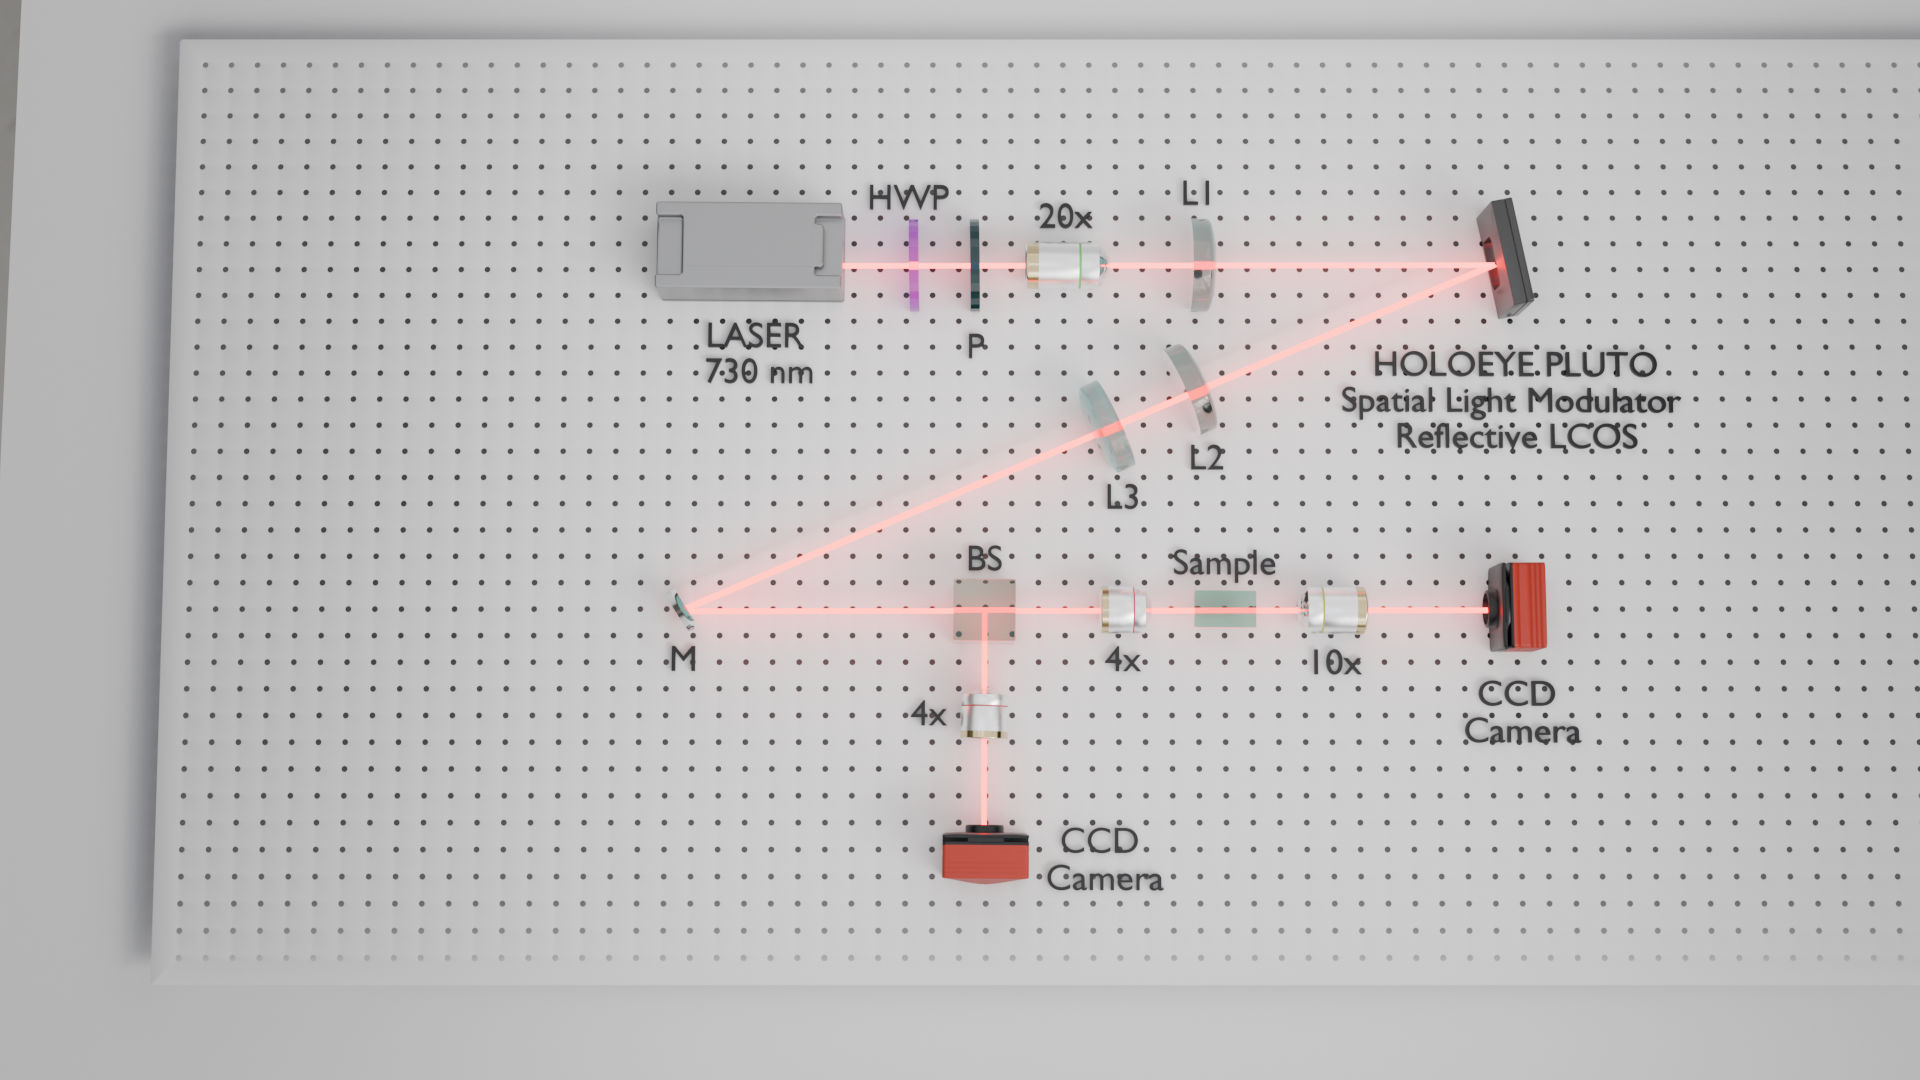
\includegraphics[width=0.8\linewidth, trim={21cm 5cm 7cm 5cm}, clip]{media/SLM_setupv1}
	\caption[Diagram of the spatial light modulation system]{Complete diagram of the experimental system for spatial light modulation, showing the optical components and their relative arrangements.}
	\label{fig:SLM_setup}
\end{figure}

\subsection{Generation of Complex Images \label{cap:oam}}
The capability for precise control over amplitude and phase is verified through the generation of optical vortices, quantified by their Orbital Angular Momentum (OAM). Interferometric analysis allows:
\begin{itemize}
	\item Determining the topological charge ℓℓ by counting the spiral branches in the interference pattern.
	\item Establishing the sign of ℓℓ through the direction of rotation of the phase front.
\end{itemize}

\begin{figure}[H]
	\centering
	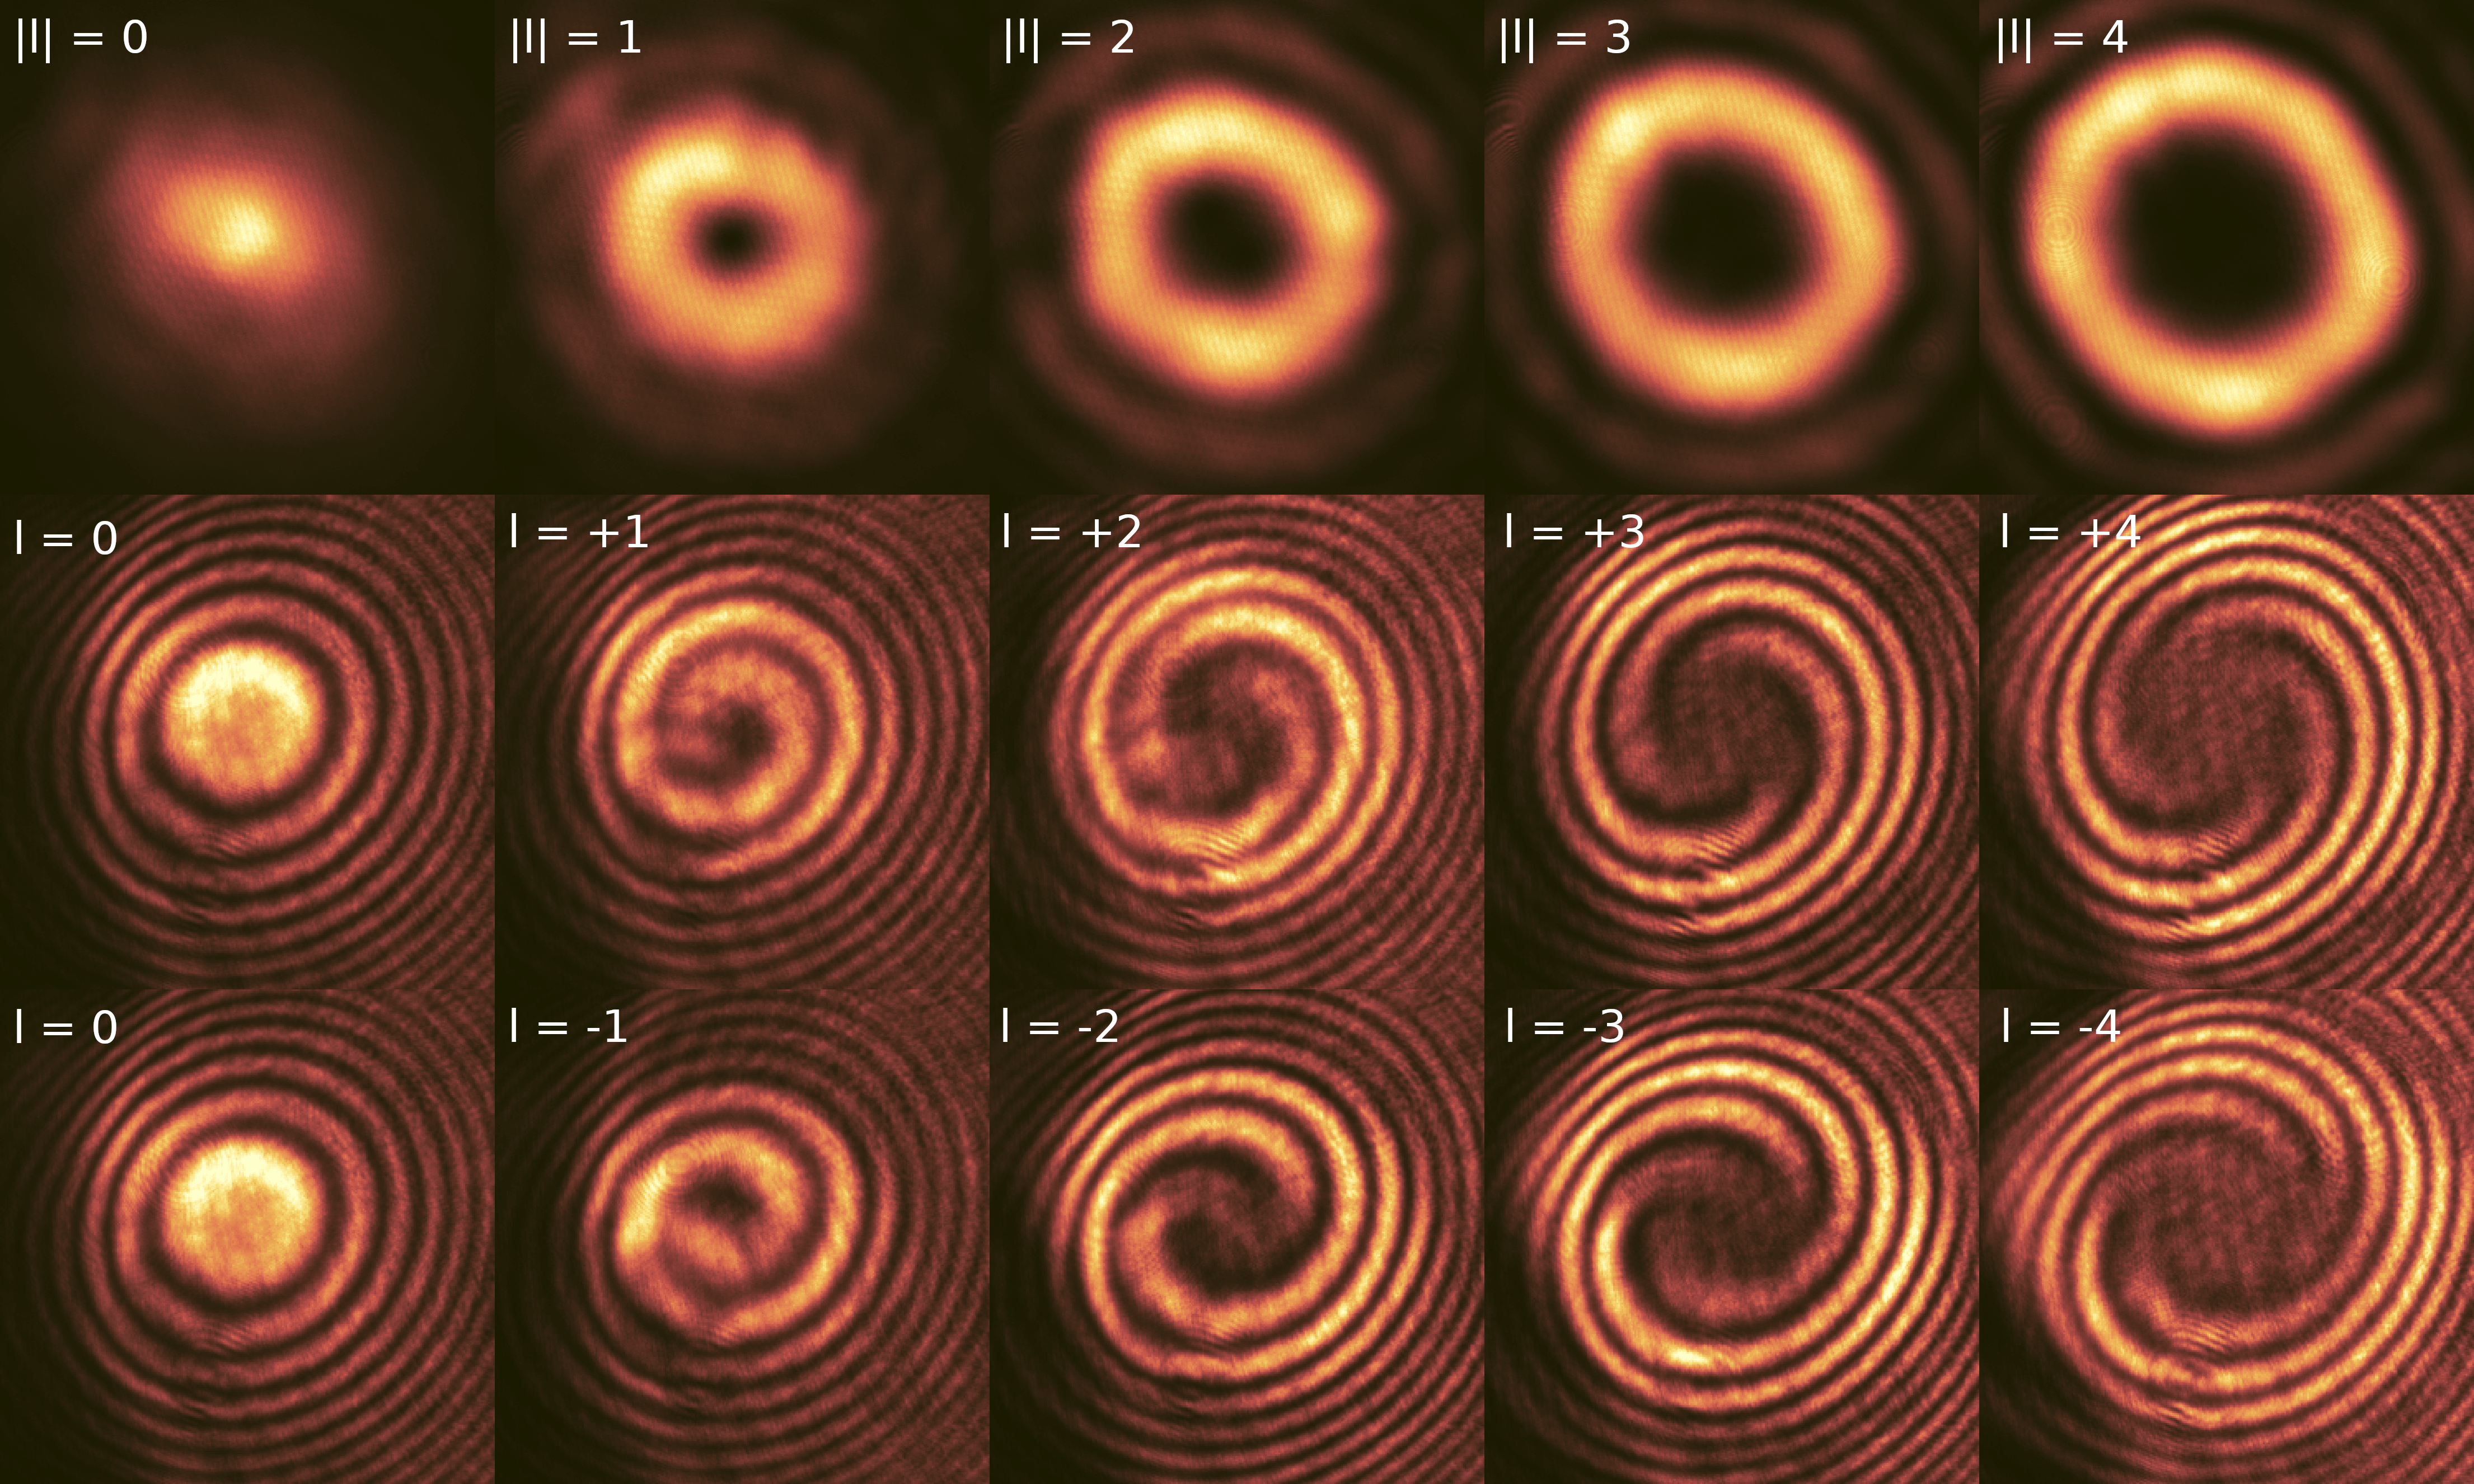
\includegraphics[width=0.8\linewidth]{media/OAM-free.png}
	\caption[Characterization of optical vortices via Mach-Zehnder interferometry.]{Characterization of optical vortices via Mach-Zehnder interferometry. \textbf{Top:} Intensity for different OAM charges ($\ell$). \textbf{Middle and Bottom:} Corresponding interference patterns, where the number of spiral branches indicates $|\ell|$ and the direction of rotation accounts for the sign of $\ell$.}
	\label{fig:OAM}
\end{figure}
\section{Image Analysis \label{sec:imageanal}}
From the captured images, it is possible to extract information about the power contained at each site of the discrete photonic system under study. To achieve this, the entire image must be divided into equally spaced rectangles that enclose the regions where waveguides are present, whether illuminated or not. The power at each site will then be the sum of the intensity of every pixel within its respective rectangle.

Image processing includes:
\begin{itemize}
	\item Background correction
	\item Normalization by maximum intensity.
	\item Automatic segmentation via thresholding.
\end{itemize}

The obtained data allow for the reconstruction of the power distribution within the photonic lattice and the analysis of coupling phenomena between neighboring waveguides.